\documentclass[11pt,twoside,a4paper]{article}
% http://www-h.eng.cam.ac.uk/help/tpl/textprocessing/latex_maths+pix/node6.html symboles de math
% http://fr.wikibooks.org/wiki/Programmation_LaTeX Programmation latex (wikibook)
%=========================== En-Tete =================================
%--- Insertion de paquetages (optionnel) ---
\usepackage[french]{babel}   % pour dire que le texte est en fran{\'e}ais
\usepackage{a4}	             % pour la taille   
\usepackage[T1]{fontenc}     % pour les font postscript
\usepackage{epsfig}          % pour gerer les images
%\usepackage{psfig}
\usepackage{amsmath, amsthm} % tres bon mode mathematique
\usepackage{amsfonts,amssymb}% permet la definition des ensembles
\usepackage{float}           % pour le placement des figure
\usepackage{verbatim}

\usepackage{longtable} % pour les tableaux de plusieurs pages

\usepackage[table]{xcolor} % couleur de fond des cellules de tableaux

\usepackage{lastpage}

\usepackage{multirow}

\usepackage{multicol} % pour {\'e}crire dans certaines zones en colonnes : \begin{multicols}{nb colonnes}...\end{multicols} 

% \usepackage[top=1.5cm, bottom=1.5cm, left=1.5cm, right=1.5cm]{geometry}
% gauche, haut, droite, bas, entete, ente2txt, pied, txt2pied
\usepackage{vmargin}
\setmarginsrb{0.20cm}{0.20cm}{0.20cm}{0.20cm}{15pt}{3pt}{15pt}{3pt}

\usepackage{lscape} % changement orientation page
%\usepackage{frbib} % enlever pour obtenir references en anglais
% --- style de page (pour les en-tete) ---
\pagestyle{empty}

% % % en-tete et pieds de page configurables : fancyhdr.sty

% http://www.trustonme.net/didactels/250.html

% http://ww3.ac-poitiers.fr/math/tex/pratique/entete/entete.htm
% http://www.ctan.org/tex-archive/macros/latex/contrib/fancyhdr/fancyhdr.pdf
% \usepackage{fancyhdr}
% \pagestyle{fancy}
% % \newcommand{\chaptermark}[1]{\markboth{#1}{}}
% % \newcommand{\sectionmark}[1]{\markright{\thesection\ #1}}
% \fancyhf{}
% \fancyhead[LE,RO]{\bfseries\thepage}
% \fancyhead[LO]{\bfseries\rightmark}
% \fancyhead[RE]{\bfseries\leftmark}
% \fancyfoot[LE]{\thepage /\pageref{LastPage} \hfill
	% TITLE
% \hfill 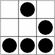
\includegraphics[width=0.5cm]{img/logo_glider.png} }
% \fancyfoot[RO]{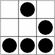
\includegraphics[width=0.5cm]{img/logo_glider.png} \hfill
	% TITLE
% \hfill \thepage /\pageref{LastPage}}
% \renewcommand{\headrulewidth}{0.5pt}
% \renewcommand{\footrulewidth}{0.5pt}
% \addtolength{\headheight}{0.5pt}
% \fancypagestyle{plain}{
	% \fancyhead{}
	% \renewcommand{\headrulewidth}{0pt}
% }

\def\imgCORPS{\begin{tabular}[h]{p{0.65cm}}\includegraphics[width=0.50cm]{../../../../../../imgGraphics/rolePlayingGame/SimulacreS/normal40x40/corps.png}		\\ \end{tabular}}
\def\imgINSTI{\begin{tabular}[h]{p{0.65cm}}\includegraphics[width=0.50cm]{../../../../../../imgGraphics/rolePlayingGame/SimulacreS/normal40x40/instinct.png}	\\ \end{tabular}}
\def\imgCOEUR{\begin{tabular}[h]{p{0.65cm}}\includegraphics[width=0.50cm]{../../../../../../imgGraphics/rolePlayingGame/SimulacreS/normal40x40/coeur.png}		\\ \end{tabular}}
\def\imgESPRI{\begin{tabular}[h]{p{0.65cm}}\includegraphics[width=0.50cm]{../../../../../../imgGraphics/rolePlayingGame/SimulacreS/normal40x40/esprit.png}		\\ \end{tabular}}

\def\imgPERCE{\begin{tabular}[h]{p{0.65cm}}\includegraphics[width=0.50cm]{../../../../../../imgGraphics/rolePlayingGame/SimulacreS/normal40x40/perception.png}	\\ \end{tabular}}
\def\imgACTIO{\begin{tabular}[h]{p{0.65cm}}\includegraphics[width=0.50cm]{../../../../../../imgGraphics/rolePlayingGame/SimulacreS/normal40x40/action.png}		\\ \end{tabular}}
\def\imgDESIR{\begin{tabular}[h]{p{0.65cm}}\includegraphics[width=0.50cm]{../../../../../../imgGraphics/rolePlayingGame/SimulacreS/normal40x40/desir.png}		\\ \end{tabular}}
\def\imgRESIS{\begin{tabular}[h]{p{0.65cm}}\includegraphics[width=0.50cm]{../../../../../../imgGraphics/rolePlayingGame/SimulacreS/normal40x40/resistance.png}	\\ \end{tabular}}

\def\imgMINER{\begin{tabular}[h]{p{0.65cm}}\vspace{1pt} \\ \includegraphics[width=0.50cm]{../../../../../../imgGraphics/rolePlayingGame/SimulacreS/normal40x40/mineral.png}	\\ \vspace{1pt} \\ \end{tabular}}
\def\imgVEGET{\begin{tabular}[h]{p{0.65cm}}\vspace{1pt} \\ \includegraphics[width=0.50cm]{../../../../../../imgGraphics/rolePlayingGame/SimulacreS/normal40x40/vegetal.png}	\\ \vspace{1pt} \\ \end{tabular}}
\def\imgANIMA{\begin{tabular}[h]{p{0.65cm}}\vspace{1pt} \\ \includegraphics[width=0.50cm]{../../../../../../imgGraphics/rolePlayingGame/SimulacreS/normal40x40/animal.png}		\\ \vspace{1pt} \\ \end{tabular}}
\def\imgHUMAI{\begin{tabular}[h]{p{0.65cm}}\vspace{1pt} \\ \includegraphics[width=0.50cm]{../../../../../../imgGraphics/rolePlayingGame/SimulacreS/normal40x40/humain.png}		\\ \vspace{1pt} \\ \end{tabular}}
\def\imgMECAN{\begin{tabular}[h]{p{0.65cm}}\vspace{1pt} \\ \includegraphics[width=0.50cm]{../../../../../../imgGraphics/rolePlayingGame/SimulacreS/normal40x40/mecanique.png}	\\ \vspace{1pt} \\ \end{tabular}}
\def\imgNEANT{\begin{tabular}[h]{p{0.65cm}}\vspace{1pt} \\ \includegraphics[width=0.50cm]{../../../../../../imgGraphics/rolePlayingGame/SimulacreS/normal40x40/neant.png}		\\ \vspace{1pt} \\ \end{tabular}}

\def\imgPUISS{\begin{tabular}[h]{p{0.65cm}}\vspace{1pt} \\ \includegraphics[width=0.50cm]{../../../../../../imgGraphics/rolePlayingGame/SimulacreS/normal40x40/puissance.png}	\\ \vspace{1pt} \\ \end{tabular}}
\def\imgRAPID{\begin{tabular}[h]{p{0.65cm}}\vspace{1pt} \\ \includegraphics[width=0.50cm]{../../../../../../imgGraphics/rolePlayingGame/SimulacreS/normal40x40/rapidite.png}	\\ \vspace{1pt} \\ \end{tabular}}
\def\imgPRECI{\begin{tabular}[h]{p{0.65cm}}\vspace{1pt} \\ \includegraphics[width=0.50cm]{../../../../../../imgGraphics/rolePlayingGame/SimulacreS/normal40x40/precision.png}	\\ \vspace{1pt} \\ \end{tabular}}


%============================= Corps =================================
\begin{document}

\begin{tabular}[h]{p{4cm} p{10cm} p{4cm}}
	Feuille de personnage \newline \emph{({\`a} photocopier)}
		&
	\begin{tabular}[h]{ p{9.5cm} }
		\includegraphics[width=9cm]{../../../../../../imgGraphics/rolePlayingGame/SimulacreS/logos/logoSimulacreS01.png} \\
	\end{tabular}
		&
	\begin{tabular}[h]{ p{2.0cm} p{2.0cm} }
		\emph{ 		 }				&	\scriptsize{R{\`e}gles de Base}	\\
									&									\\
									&									\\
									&									\\
		\emph{Univers : } \newline	&	\emph{ 		 }					\\
	\end{tabular}
		\\
\end{tabular}

\begin{tabular}[h]{|p{3.5cm}|p{3.5cm}|p{3.5cm}|p{3.5cm}|p{3.5cm}|}
	\hline
		\multicolumn{4}{|p{14cm}|}{\emph{Nom du personnage : }} 
			& \multicolumn{1}{ p{3.5cm}|}{\emph{{\^A}ge : }} \\
	\hline
		\multicolumn{2}{|p{7cm}|}{\emph{Race : }} 
			& \multicolumn{1}{ p{3.5cm} }{\emph{Sexe : }} 
			& \multicolumn{2}{|p{7cm}|}{\emph{M{\'e}tier : }} \\
	\hline
		\multicolumn{1}{ p{4cm} }{  }
					&	\multicolumn{2}{ p{7cm} }{\emph{Nom du joueur : }}
					& 	\multicolumn{2}{ p{7cm} }{\emph{Date de cr{\'e}ation : }} \\
\end{tabular}~\\

\begin{tabular}[h]{ p{5cm} p{1.0cm} p{5cm}  p{1.0cm} p{6cm} }

{\centering \emph{Composantes}}		& {\scriptsize \emph{3 {\`a} 6 \newline (18pts)} }	
	&	{\centering \emph{Moyens}}	& {\scriptsize \emph{0 {\`a} 4 \newline (10pts)} }	
	& 	
\multirow{3}{5cm}{% 
	\begin{tabular}[h]{|p{5.0cm}|}%
		\hline												%
		\emph{Dessin ou description}						\\	%
		\fbox{ \resizebox{4.60cm}{9.0cm}{ \mbox{ . } } }	\\	%
		\scriptsize{Vie	(PV)						\hfill 	\_ / 4 (6)}		\\	% 
		\scriptsize{Souffle	(PS)					\hfill	\_ / 4 (6)}		\\	% 
		\scriptsize{{\'E}quilibre psychique	(EP)	\hfill	\_ / 4 (6)}		\\	% 
		\scriptsize{Armure					\hfill	\_\_ / \_\_ / \_\_}		\\	% 
		\scriptsize{	\hfill	[ Protection / G{\^e}ne / Absorption ] }	\\	% 
		\hline												%
	\end{tabular}%
} \\

\multicolumn{2}{ p{6.0cm} }{ 
	{\footnotesize %
	\begin{tabular}[h]{|p{0.75cm}|p{3.0cm}|p{0.25cm}|p{0.50cm}|}
		\hline
		\imgCORPS & CORPS & \begin{tabular}[c]{|p{0.20cm}|}
		 \\ \hline \\ \hline \\
		\end{tabular} & --- \\
		\hline
		\imgINSTI & INSTINCT & \begin{tabular}[c]{|p{0.20cm}|}
		 \\ \hline \\ \hline \\
		\end{tabular} & --- \\
		\hline
		\imgCOEUR & C\OE UR & \begin{tabular}[c]{|p{0.20cm}|}
		 \\ \hline \\ \hline \\
		\end{tabular} & --- \\
		\hline
		\imgESPRI & ESPRIT & \begin{tabular}[c]{|p{0.20cm}|}
		 \\ \hline \\ \hline \\
		\end{tabular} & --- \\
		\hline
	\end{tabular} }
}	& 
\multicolumn{2}{ p{6.0cm} }{ 
	{\footnotesize %
	\begin{tabular}[h]{|p{0.75cm}|p{3.0cm}|p{0.75cm}|}
		\hline
		\vspace{0.05pt} & & \\
		\imgPERCE &  PERCEPTION		 & --- \\
		\hline
		\vspace{0.05pt} & & \\
		\imgACTIO &  ACTION			 & --- \\
		\hline
		\vspace{0.05pt} & & \\
		\imgDESIR &  D{\'E}SIR		 & --- \\
		\hline
		\vspace{0.05pt} & & \\
		\imgRESIS &  R{\'E}SISTANCE	 & --- \\
		\hline
		\multicolumn{3}{ p{6cm} }{ \rule{0.25\textwidth}{0.25mm} }	\\
		\multicolumn{3}{ p{6cm} }{ \rule{0.15\textwidth}{0.25mm} }	\\
	\end{tabular} }
}	& \hfill \\

\multicolumn{4}{ p{12.0cm} }{
	\begin{tabular}[h]{ p{11.5cm} }
		\\
		\emph{R{\^e}gnes}
		{\scriptsize \emph{0 {\`a} 2 ; (08pts pour R{\^e}gnes et {\'E}nergies )} }  \\
		{\footnotesize %
		\begin{tabular}[h]{|p{0.75cm}|p{1.75cm}|p{0.50cm}|p{0.75cm}|p{1.75cm}|p{0.50cm}|p{0.75cm}|p{1.75cm}|p{0.50cm}|}
			\hline
			\imgMINER & Min{\'e}ral		& --- & \imgVEGET & V{\'e}g{\'e}tal		& --- & \imgANIMA & Animal		& --- \\
			\hline
			\imgHUMAI & Humain			& --- & \imgMECAN & M{\'e}canique		& --- & \imgNEANT & N{\'e}ant	& \textbf{-1} \\ 
			\hline
		\end{tabular} } \\
		\\
		\emph{{\'E}nergies de base} \\
		{\footnotesize %
		\begin{tabular}[h]{|p{0.75cm}|p{1.75cm}|p{0.50cm}|p{0.75cm}|p{1.75cm}|p{0.50cm}|p{0.75cm}|p{1.75cm}|p{0.50cm}|}
			\hline
			\imgPUISS & Puissance		& --- & \imgRAPID & Rapidit{\'e}		& --- & \imgPRECI & Pr{\'e}cision	& --- \\
			\hline
		\end{tabular} } \\
	\end{tabular}
}% 
& \\
\end{tabular}

~\\

{\scriptsize %
\begin{tabular}[h]{ p{12cm} p{6cm} }
	\textbf{\emph{Armes}} &  \\
	\begin{tabular}[h]{|p{5.0cm}|p{2.5cm}|p{4.5cm}|}
		\hline
			{\centering \emph{Nom de l'arme} }	&
			{\centering \emph{D{\'e}g{\^a}ts} }	&
			{\centering \emph{Note} }			\\
		\hline
			\dotfill & 
			[~~] PV, [~~] PS				& 
			\dotfill	\\
		\hline
			\dotfill	& 
			[~~] PV, [~~] PS				& 
			\dotfill	\\
		\hline
			\dotfill	& 
			[~~] PV, [~~] PS				& 
			\dotfill	\\
		\hline
	\end{tabular}
	& 
	\begin{tabular}[h]{ p{1.0cm}|p{5.0cm}|}
		\cline{2-2}
		 & \emph{Capacit{\'e}s sp{\'e}ciales}		\\
		\cline{2-2}
		 & \dotfill		\\
		\cline{2-2}
		 & \dotfill		\\
		\cline{2-2}
		 & \dotfill		\\
		\cline{2-2}
	\end{tabular}
	\\
\end{tabular} }

~\\

\begin{tabular}[h]{|p{9.25cm}|p{9.25cm}|}
	\hline
	\textbf{\emph{Technique de jeu}	}	&
	\textbf{\emph{Histoire}			}	\\
	\hline
	\emph{M{\'e}tiers, Talents et Hobbies}
	\newline	\newline	\newline	\newline	\newline
	\rule{0.4\textwidth}{0.25mm}
	\emph{Objets transport{\'e}s}
	\newline	\newline	\newline	\newline	\newline
		&
	\emph{Pass{\'e} du personnage}
	\newline	\newline	\newline	\newline	\newline
	\rule{0.4\textwidth}{0.25mm}
	\emph{Notes sur l'aventure actuelle}
	\newline	\newline	\newline	\newline	\newline
		\\
	\hline
\end{tabular}


~\\

\end{document}
